\section{\gls{ims} dataset No.1 - Bearing 3x sensor}
\label{sec:ValidationOnRealWorldData}
\begin{figure}
    \centering
    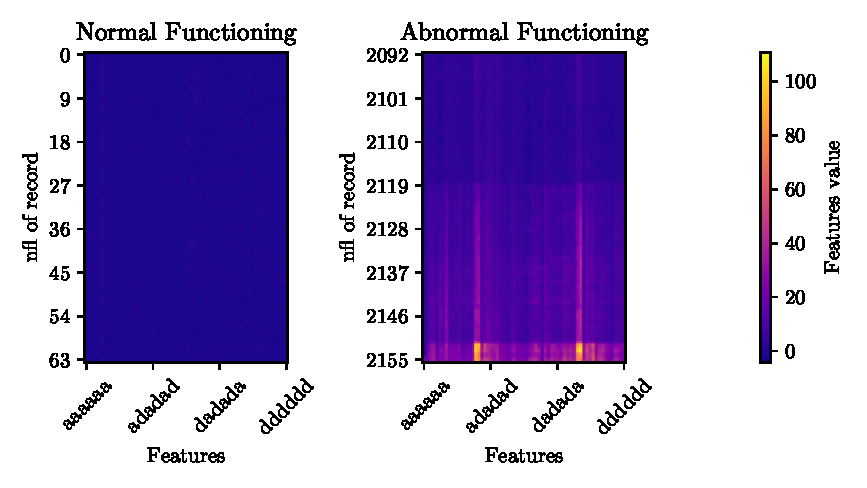
\includegraphics{images/IMS/Heatmap.pdf}
    \caption{Heatmap of the standardized features value for the test $\text{n}^\circ$1 of \gls{ims} dataset}
    \label{fig:Heatmap}
\end{figure}


To start the validation, let's subdivide the test No.1 of the \gls{ims} dataset into training and testing datasets. The first 500 samples are used for training, and the remaining samples are used for testing. The configuration file is set to use the data from the \quoted{bearing 3x} sensor, extracting all the time-domain and frequency-domain features described in \autoref{ch:FeatureExtraction}. The training dataset is used to train the \gls{mla} to recognize the normal behavior of the bearing, and the testing dataset is used to validate the trained model. The \autoref{tab:IMS_test_parameters} shows the parameters of the test No.1 of the \gls{ims} dataset. For display purposes, the features are standardized, and the heatmap of the standardized features is shown in \autoref{fig:Heatmap} in normal and abnormal conditions.

The abstract version of the \gls{fieldAg} has been used to extract the features from the dataset, creating all the snapshots in the set $\gls{sym:snapset}=\{\gls{sym:snap}_1,\gls{sym:snap}_2,\dots,\gls{sym:snap}_{500}\}$. Theese snapshots are stored in the \emph{unconsumed} collection of the database.

\subsection{Training - K-means}

Using the commands of the \gls{cli}, the training procedure has been launched:
\begin{minted}[linenos,breaklines]{bash}
    C:/Users/JohnSmith/Code/framework> python ./MASTER.py run-feature-agent
    C:/Users/JohnSmith/Code/framework> python ./MASTER.py run-machine-learning-agent novelty train
\end{minted}

where the first command runs the \gls{fieldAg} and the second one runs an \quoted{healthy} instance of the \gls{mla} in training mode.
At this point, the \gls{mla} ask the user to move the snapshots from the \emph{unconsumed} to the \emph{healthy} colection, since the \emph{healthy} collection is empty. After the confirmation, the \gls{mla} starts the training with different number of clusters, and output the scoring in the form of silhouette and inertia scores. The results are shown in \autoref{fig:SilScore_01} and \autoref{fig:InertiaScore_01}. The user can confirm that the best number of clusters is 2, as the silhouette score is the highest and the inertia score is at the \gls{pof} point, or insert another number of clusters, rememebering that it is best to overestimate the number of clusters to increase the system sensitivity, as discussed in \autoref{sec:wrong_k}. 

In this case the number of cluster has been set to 2, so that the \gls{mla} saves the model trained with $n=2$ into the database. Even if the feature space has high dimensionality, the agent plot to the user also a scatter plot of a subset of features of the training dataset, to have a visual feedback of the clustering, as shown in \autoref{fig:Clusters}, where the points are the snapshots, the crosses are the centroids and the colors represent the assigned cluster. We can observe that selecting 2 as the number of clusters is adequate and that the projections of the clusters shapes on some planes are not perfectly spherical but, at least, they are not too elongated. This is a good sign for the K-means algorithm, as discussed in \autoref{sec:kmeans_limits}.

\begin{figure}
    \centering
    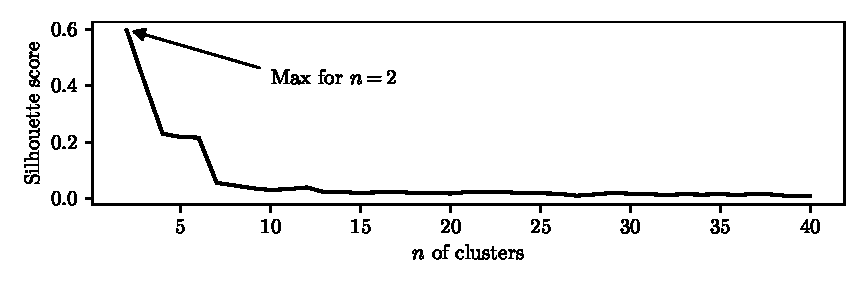
\includegraphics{images/IMS/SilScore_01.pdf}
    \caption{Silhouette score for clustering the test $\text{n}^\circ$1 of \gls{ims} dataset (K-means)}
    \label{fig:SilScore_01}
\end{figure}

\begin{figure}
    \centering
    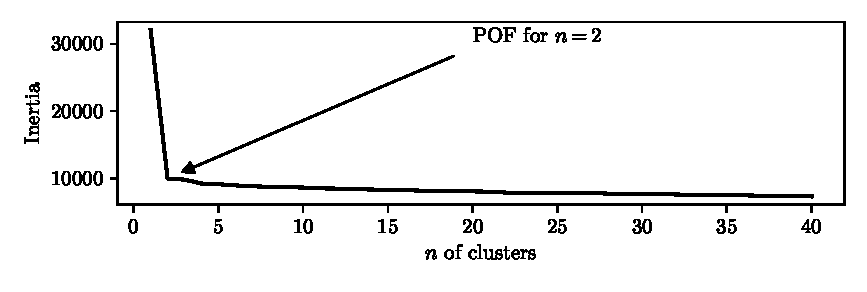
\includegraphics{images/IMS/InertiaScore_01.pdf}
    \caption{Inertia score for clustering the test $\text{n}^\circ$1 of \gls{ims} dataset (K-means)}
    \label{fig:InertiaScore_01}
\end{figure}

\begin{figure}
    \centering
    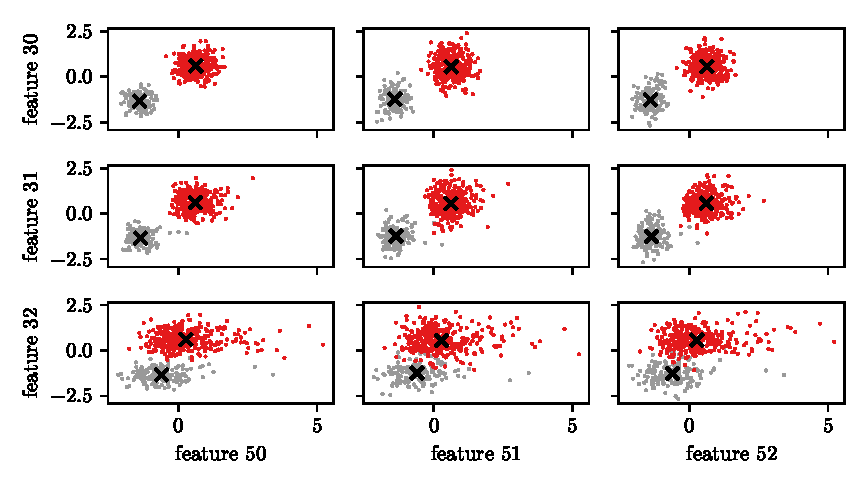
\includegraphics{images/IMS/Clusters.pdf}
    \caption{Scatterplot of training $\gls{glo:snap}$ for the test $\text{n}^\circ$1 of \gls{ims} dataset}
    \label{fig:Clusters}
\end{figure}

\subsection{\gls{nd} Validation - K-means}
Using the validation partition of the dataset, it is possible to set the \gls{mla} in \emph{evaluate} mode. The \gls{fieldAg} uses the validation partition and fill the \emph{raw} collection with the timeseries. The {\gls{fa}} extract the features and continuously fill the \emph{unconsumed} collection with the snapshots. The \gls{mla} evaluates the snapshots according to \autoref{alg:eval_new_snapshot}  and plots the result, as well as generating a warning if the novelty metric is greater than a certain threshold. The results are shown in \autoref{fig:NoveltyScore_01}, where we can see that the framwork detects the novelty quite early, at 2003-11-16 07:46, while the dataset authors, declared the test finished because of bering defects (not catastrofic failures) at 2003-11-25 23:40. The comparision of the margin of early detection for different algorithms will be resumed later.

\begin{figure}
    \centering
    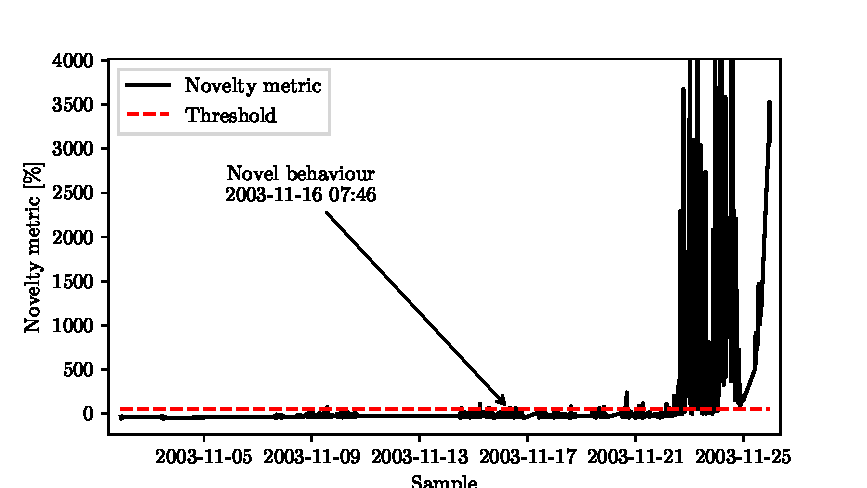
\includegraphics{images/IMS/Novelty_01_500samples_bearing3x.pdf}
    \caption{Results of \gls{nd} for the test $\text{n}^\circ$1 of \gls{ims} dataset (K-means)}
    \label{fig:NoveltyScore_01} 
\end{figure}

\subsection{Training - \gls{dbscan}}
Using the same partition of dataset as for the K-means training, we can train a \gls{dbscan} model. In this case the silhouette score have to be used to select a suitable value of the radius $\varepsilon$. As shown in \autoref{fig:silscore_dbscan}, the optimal value is 8, that corresponds correctly to the generation of two clusters.

\begin{figure}
    \centering
    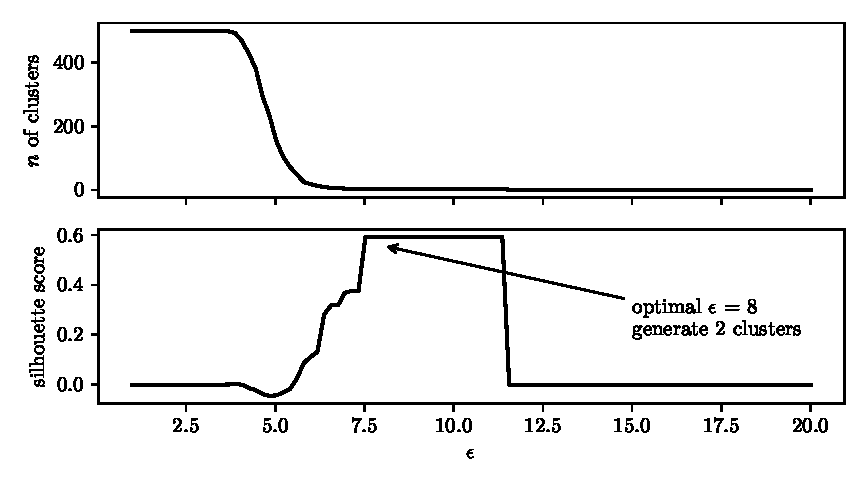
\includegraphics{images/IMS/InertiaScore_01_dbscan.pdf}
    \caption{Silhouette score for clustering the test $\text{n}^\circ$1 of \gls{ims} dataset (\gls{dbscan})}
    \label{fig:silscore_dbscan}
\end{figure}

\subsection{\gls{nd} Validation - \gls{dbscan}}
As it has been done for the K-means, the validation partition of the dataset is now used for performing \gls{nd} with the \gls{dbscan} model, as described in \autoref{sec:dbscan_eval}. The result is shown in \autoref{fig:NoveltyScore_01_dbscan}, where we can see that the \gls{dbscan} model detects the novelty at 2003-11-22 15:06, that is quite early, but not as early as the K-means model. This is because the metric generated by the \gls{dbscan} model have a greater variance so, instead of increasing consistently, it overshoot the threshold quite before this time, but fails to consistently stay above the threshold. 

\begin{figure}
    \centering
    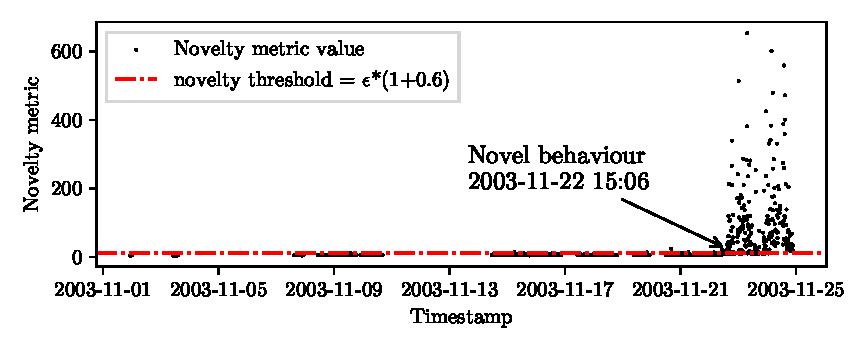
\includegraphics{images/IMS/Novelty_01_500samples_bearing3x_dbscan.pdf}
    \caption{Results of \gls{nd} for the test $\text{n}^\circ$1 of \gls{ims} dataset (\gls{dbscan})}
    \label{fig:NoveltyScore_01_dbscan}
\end{figure}

\subsection{Training -\gls{gmm}}
Let's now try with the \gls{gmm} model. The metric for selecting the number of cluster are now the \gls{bic} and the \gls{aic}, as shown in \autoref{fig:bic_aic_gmm} and \autoref{fig:aic_gmm}. The  two metrics diverges but, as discussed in \autoref{sec:gauss_train}, the \gls{aic} tends to perform better. In this case, minimizing the \gls{aic} leads to select 25 as the number of clusters, that is much more than what selected with the K-means, but still a reasonable choice, also considering that the \gls{gmm} is a soft clustering algorithm and that we are using the density as a metric to perform \gls{nd}.

\begin{figure}
    \centering
    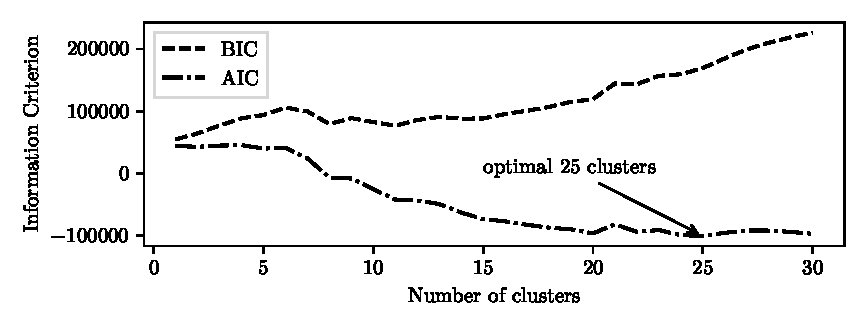
\includegraphics{images/IMS/BICAIC_GMM.pdf}
    \caption{\gls{bic} and \gls{aic} for clustering the test $\text{n}^\circ$1 of \gls{ims} dataset (\gls{gmm})}
    \label{fig:bic_aic_gmm}
\end{figure}

\subsection{\gls{nd} Validation - \gls{gmm}}
The validation partition of the dataset is now used for performing \gls{nd} with the \gls{gmm} model. The result is shown in \autoref{fig:NoveltyScore_01_gmm}, where we can see that the \gls{gmm} model detects the novelty at 2003-11-22 03:47. The consideration about this result are the same as for the \gls{dbscan} model. In \autoref{fig:NoveltyScore_01_gmm}, the metric (density value) appears in colored dots, as each color represent the cluster to which the snapshot has been assigned.
\begin{figure}
    \centering
    \includegraphics{images/IMS/Novelty_01_500samples_bearing3x_gmm.pdf}
    \caption{Results of \gls{nd} for the test $\text{n}^\circ$1 of \gls{ims} dataset (\gls{gmm})}
    \label{fig:NoveltyScore_01_gmm}
\end{figure}